\section{Analysis}
\label{sec:analysis}
%(2 pages)

\begin{figure*}
  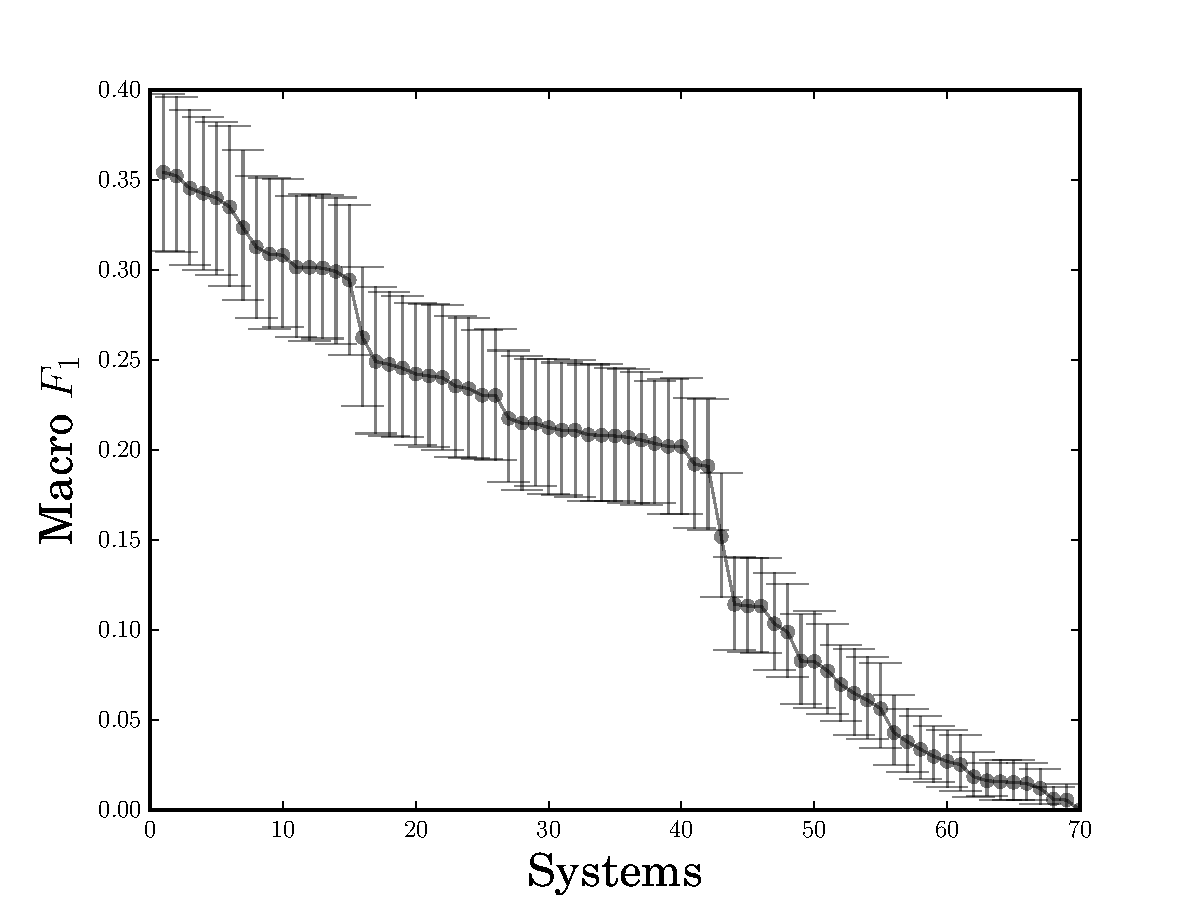
\includegraphics[width=\columnwidth]{figures/experiment1}
  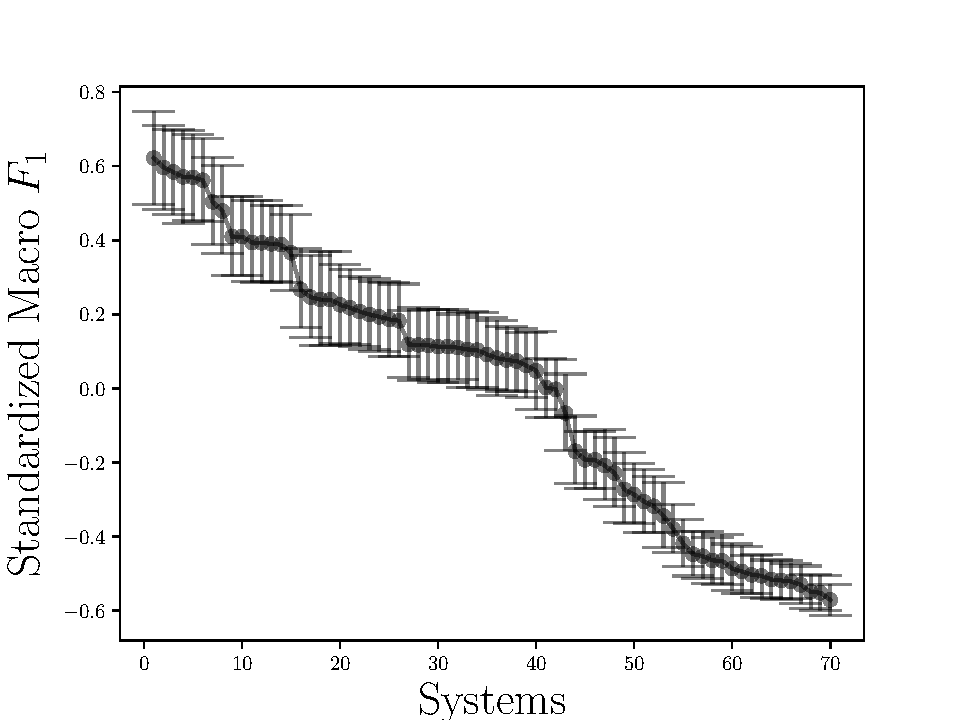
\includegraphics[width=\columnwidth]{figures/experiment3}
  \caption{Evaluating KBP}
\end{figure*}

This section, we perform an analysis.

Describe our dataset that we have to work with -- what is evaluated and what is not.

Dataset statistics. -- number of documents, queries, submissions; heatmap of submission x query.

Assume that systems by the same university are more similar and group by that axes?

\subsection{Are we improving over time?}

\paragraph{Standardizing scores for comparison.}

Describe linear model.
Correct for variation across queries.

\paragraph{Results.}

Graphs of performance before and after standardization.

Decode what aspects we are actually improving on.


\begin{figure}
  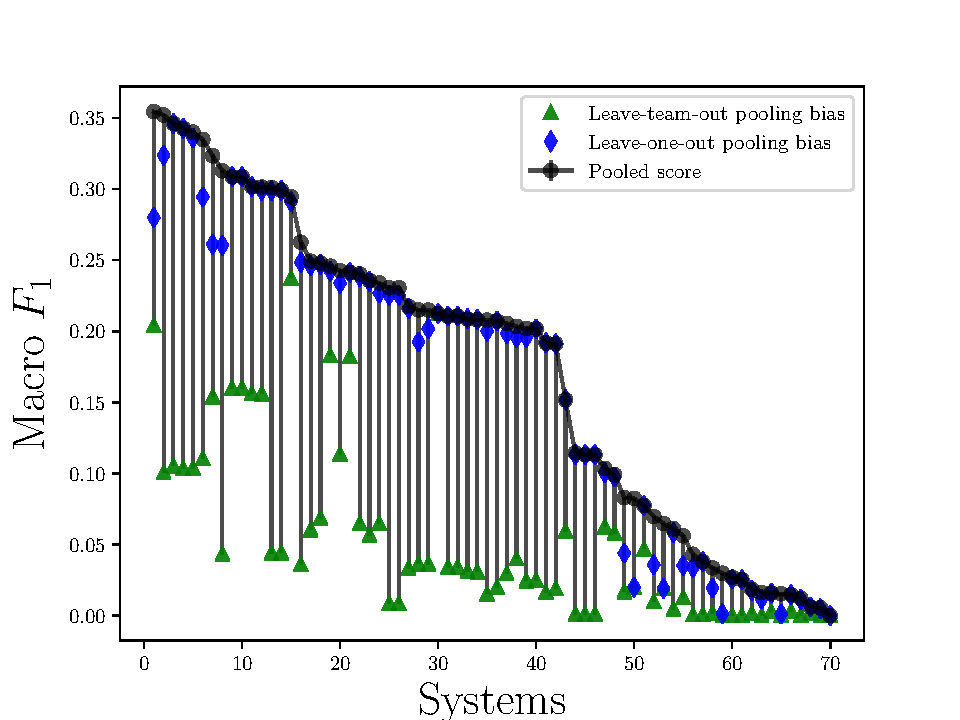
\includegraphics[width=\columnwidth]{figures/experiment2}
  \caption{Pooling bias.}
\end{figure}


\subsection{Are we biased against improvements?}

\paragraph{Measuring pooling bias.}
Define pooling bias. Statistical model used.

\paragraph{Evaluating contributions of features over time.}

